\documentclass[10pt,a4paper,final]{article}
\usepackage[utf8]{inputenc}
\usepackage[french]{babel}
\usepackage[T1]{fontenc}
\usepackage{amsmath}
\usepackage{amsfonts}
\usepackage{amssymb}
\usepackage{listings}
\usepackage{fancyhdr}
\usepackage{graphicx}
\usepackage{xcolor}
\author{Léo Boisson}
\setlength\parindent{24pt}
\title{\textbf{Compte rendu TP2/3 Réseau}}
\makeindex
\pagestyle{fancy}
\lhead{BOISSON Léo}
\rhead{Compte-rendu TP Réseau}
\cfoot{\thepage}
\renewcommand{\headrulewidth}{0.4pt}
\renewcommand{\footrulewidth}{0.4pt}

\lstset{language=C,
                basicstyle=\footnotesize,
                keywordstyle=\color{blue}\ttfamily,
                stringstyle=\color{red}\ttfamily,
                keywordstyle=\bfseries\color{green!40!black},
                commentstyle=\itshape\color{purple!40!black},
                identifierstyle=\color{blue},
                breaklines=true,
				frame=trbl,
				numbers=left,
 				xleftmargin=\parindent,
                morecomment=[l][\color{magenta}]{\#}
}

\begin{document}
\date{}
\maketitle  
\tableofcontents  
\newpage



\section{Introduction} 

	\subsection{Historique}
		Les sockets sont un ensemble de fonctions de communications, proposés en 1980 pour le \textbf{Berkeley Software Distribution} (BSD), en open source, par 								l'université de Berkeley. Elles permettent a des applications de se connecter entre elles, via un principe client/serveur.	\\
		Aujourd'hui, les sockets sont disponibles dans quasiment tous les langages de programmations, et font offices de norme.\\
		On distingue deux modes de communication avec les sockets :\\
		\begin{itemize}
			\item
				Le mode connecté, qui utilise le protocole TCP. Dans ce mode, une connexion durable est établie entre les deux processus, afin que l'adresse de destination ne 							soit pas nécessaire à chaque envoie de données.
			\item
				Le mode non-connecté, qui utilise le protocole UDP. Ce mode nécessite l'adresse de destination à chaque envoi, et il n'y a pas de confirmation du bon envoi des
				données. Ce mode est plus adapté à l'envoi de flux audio ou vidéo.
		\end{itemize}+
		
	\subsection{Objectif du TP}
		L'objectif de ce TP est d'aborder le développement de sockets, et de se familiariser avec les outils qui vont avec (les primitives). Pour cela, nous allons 
		programmer des applications client/serveur basique, pour ensuite observer et analyser les échanges de données entre ces applications.
	
	
\section{Application client/serveur echo}
	\subsection{principe de fonctionnement}
		Nous réalisons une application de type client/serveur, afin de calculer le temps que mets une requête du client à parvenir au serveur, à être traitée, puis à revenir au 				client. Nous utilisons la primitive \textit{\textrm{gettimeofday}}, qui renvoie l'heure en secondes et microsecondes (avec la zone temporelle passée en argument).\\
		En utilisant cette fonction deux fois dans le code du client, une première fois lors de l'envoi au serveur, et une seconde lors de la réception depuis le serveur, il nous 				suffit de soustraire la première à la seconde pour obtenir le temps d'aller et retour d'une requête.
				
	\subsection{Code source du client}
		On constateras les \textit{\textrm{gettimeofday}}, lignes 81 et 104.
		\lstinputlisting{client_echo.c}
		
	\subsection{Code source du serveur}
		Le serveur ne fait que réceptionner le message du client, un "echo", et le renvoi immédiatement.
		\lstinputlisting{server_echo.c}

	\subsection{Analyse des trames réseau}
		Les programmes affichent ceci dans le terminal :\\
		
		\begin{figure}[!h] 
			\centering
			\caption{Pour le serveur :}
			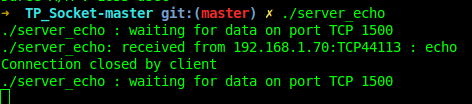
\includegraphics[scale=0.5]{img/server_echo_terminal.png} 
			\caption{Pour le client :}
			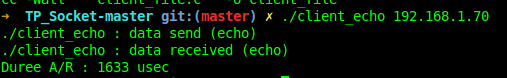
\includegraphics[scale=0.5]{img/client_echo_terminal.png} 
		\end{figure}
		\newpage
		
		Ensuite, nous regardons les trames échangées avec wireshark, en utilisant un filtre sur le port. Nous obtenons ceci :\\
		\begin{figure}[!h] 
			\centering
			\caption{Affichage dans wireshark :}
			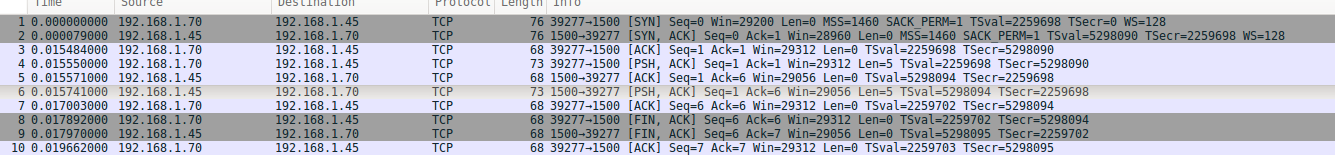
\includegraphics[scale=0.3]{img/wireshark_echo.png} 
		\end{figure}		
		\newline
		Que nous pouvons analyser plus facilement en utilisant l'option \textit{\textrm{flowchart}} dans wireshark :\\
		\begin{figure}[!h] 
			\centering
			\caption{Flowchart de echo :}
			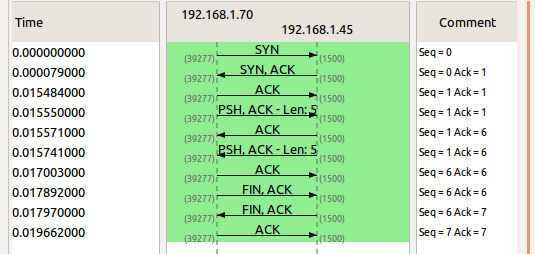
\includegraphics[scale=0.5]{img/flowchart_echo.png} 
		\end{figure}	
		\newline
		Les trois premiers paquets correspondent au mécanisme de \textit{\textrm{handshake}}. Ensuite, on voit un paquet de taille 5 aller du client au serveur. Il s'agit
		du "echo" (4 caractères + le retour chariot).\\
		\newline
		Ensuite, le serveur envoi l'accusé de réception, avec le numéro d'acquittement 6 (5+1), puis il envoi la sa réponse à la requête, soit le message "echo".
		le numéro d'acquittement n'as pas changé, puisque le serveur n'as pas reçu d'autre données entre temps. \\
		S’en suit alors le paquet 7 envoyé par le client qui accuse réception du retour effectué par le serveur. Le numéro d’acquittement est devenu 6 (1+6) pour le 
		client (il a reçu 5 caractères).\\
		\newline
		Le client engage alors le processus de terminaison de la connexion. Il envoie un paquet vide avec le drapeau FIN. Le serveur lui renvoie 
		alors un paquet similaire en incrémentant le numéro d’acquittement de 1. Enfin, un dernier paquet est transmis au serveur par le client en tant qu'accusé de 
		réception du retour du paquet FIN. La connexion est alors terminée.\\
		\newpage		
		
\section{Application client/serveur chifoumi}
	\subsection{Principe du chifoumi}
		Le but de ce programme est de faire jouer l'utilisateur, par l'application client, contre le serveur. Le client enverras son choix, pierre, feuille, ou ciseaux,
		au serveur, et le serveur choisiras aléatoirement l'un des 3. \\
		On affiche les scores, et la partie se finie au bout de 3 victoires, après quoi la connexion seras perdue.

	\subsection{Code source du client}
		\lstinputlisting{q11_client.c}

	\subsection{Code source du serveur}
		\lstinputlisting{q11_server.c}

	\subsection{Analyse des trames réseau}
		Voici ce qu'afficheras le client (pour le premier tour de jeu) :\\
		
		\begin{figure}[!h] 
			\centering
			\caption{client chifoumi :}
			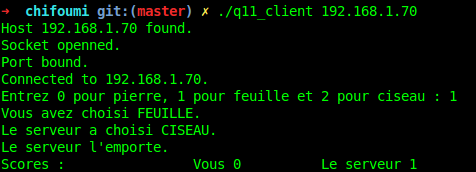
\includegraphics[scale=0.5]{img/chifoumi_terminal.png} 
		\end{figure}
		\newpage
		On peut regarder ensuite le flowchart de wireshark pour cet échange :\\
		\begin{figure}[!h] 
			\centering
			\caption{flowgraph de l'echange :}
			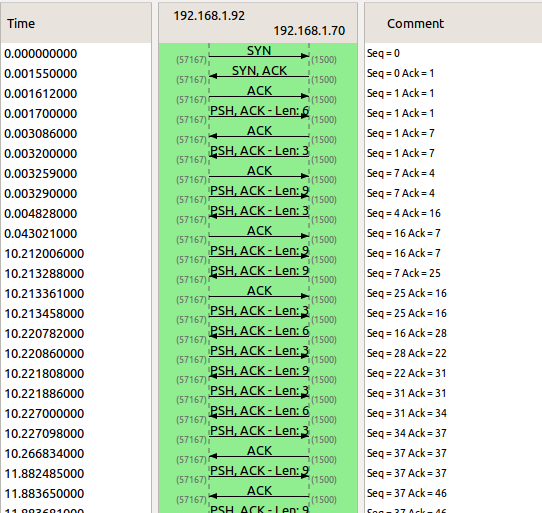
\includegraphics[scale=0.6]{img/chifoumi_flowgraph.png} 
		\end{figure}		
		\\
		Comme précédemment, les trois premiers échanges correspondent au mécanisme de \textit{\textrm{handshake}}. Ensuite, on constate les échanges de "HELLO", et "CHIFOUMI", 
		toujours suivis d'un message d'"acknowledgement".
		

\section{Échange de données entre deux machines en UDP}

	\subsection{Objectif}
		Le but de cette partie est d'échanger des chaines de caractères entre deux machine, avec une application client/serveur, et en utilisant le protocole UDP.\\
		Comme il est dit dans l'introduction, ce mode nécessiteras l'adresse de destination pour chaque envoi de données. Il n'y aura pas non plus d'accusé de réception.

	\subsection{Code source du client}
		\lstinputlisting{UDP/appliclient.c}

	\subsection{Code source du serveur}
		\lstinputlisting{UDP/appliserveur.c}

	\subsection{Analyse par Wireshark}
		Depuis la machine avec le serveur, on obtient ceci (en exécutant "./client 192.168.1.45 1500 abcde" sur la machine avec le client) :\\
		\begin{figure}[!h] 
			\centering
			\caption{serveur UDP :}
			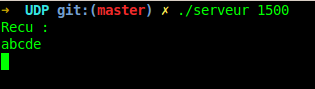
\includegraphics[scale=0.5]{img/terminal_UDP.png} 
		\end{figure}
		\\
		Puis on regarde à l'aide de wireshark les données utiles transmises :\\
		\begin{figure}[!h] 
			\centering
			\caption{wireshark UDP :}
			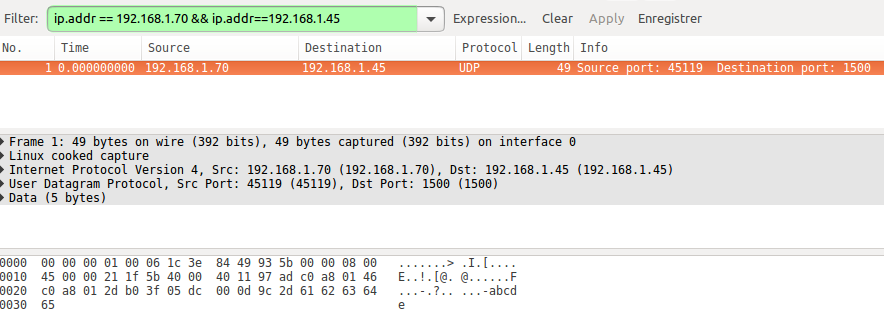
\includegraphics[scale=0.4]{img/wireshark_UDP.png} 
		\end{figure}		
		\\
		On constate que l'on a bien 5 bytes de données transmis, qui correspondent aux 5 derniers octets transmis : on voit qu'il s'agit du code ASCII hexadécimal des lettres 
		abcde.\\


\section{Conclusion}


	Lors de ce TP, la principale difficulté que j'ai rencontré à été que j'ai voulu rentrer tout de suite dans le code, sans être parfaitement à l'aise avec la théorie de 
	ces protocoles. Ce qui m'as le plus aidé à été d'écrire sur une feuille le déroulement des échanges (pour le protocole TCP).\\
	Ce TP m'auras servi à comprendre le fonctionnement des sockets, et à savoir utiliser leurs primitives. Le fait de regarder plus précisément les échanges avec Wireshark
	à également aidé à expliciter les différences entre les protocoles.



\end{document}s